\documentclass[bimj,fleqn]{w-art}
\usepackage{times}
\usepackage{w-thm}
\usepackage[authoryear]{natbib}
\usepackage{amsfonts}
\usepackage{epstopdf}
\usepackage{graphicx, latexsym}
\usepackage{color}

% \setlength{\bibsep}{2pt}
% \setlength{\bibhang}{2em}
% \newcommand{\J}{J\"{o}reskog}
% \newcommand{\So}{S\"{o}rbom}
% \newcommand{\bcx}{{\bf X}}
% \newcommand{\bcy}{{\bf Y}}
% \newcommand{\bcz}{{\bf Z}}
% \newcommand{\bcu}{{\bf U}}
% \newcommand{\bcv}{{\bf V}}
% \newcommand{\bcw}{{\bf W}}
% \newcommand{\bci}{{\bf I}}
% \newcommand{\bch}{{\bf H}}
% \newcommand{\bcb}{{\bf B}}
% \newcommand{\bcr}{{\bf R}}
% \newcommand{\bcm}{{\bf M}}
% \newcommand{\bcf}{{\bf F}}
% \newcommand{\bcg}{{\bf G}}
% \newcommand{\bcs}{{\bf S}}
% \newcommand{\bca}{{\bf A}}
% \newcommand{\bcd}{{\bf D}}
% \newcommand{\bcc}{{\bf C}}
% \newcommand{\bce}{{\bf E}}
% \newcommand{\ba}{{\bf a}}
% \newcommand{\bb}{{\bf b}}
% \newcommand{\bc}{{\bf c}}
% \newcommand{\bd}{{\bf d}}
% \newcommand{\bx}{{\bf x}}
% \newcommand{\by}{{\bf y}}
% \newcommand{\bz}{{\bf z}}
% \newcommand{\bu}{{\bf u}}
% \newcommand{\bv}{{\bf v}}
% \newcommand{\bh}{{\bf h}}
% \newcommand{\bl}{{\bf l}}
% \newcommand{\be}{{\bf e}}
% \newcommand{\br}{{\bf r}}
% \newcommand{\bw}{{\bf w}}
% \newcommand{\de}{\stackrel{D}{=}}
% \newcommand{\bt}{\bigtriangleup}
% \newcommand{\bfequiv}{\mbox{\boldmath $\equiv$}}
% \newcommand{\bmu}{\mbox{\boldmath $\mu$}}
% \newcommand{\bnu}{\mbox{\boldmath $\nu$}}
% \newcommand{\bxi}{\mbox{\boldmath $\xi$}}
% \newcommand{\btau}{\mbox{\boldmath $\tau$}}
% \newcommand{\bgamma}{\mbox{\boldmath $\Gamma$}}
% \newcommand{\bphi}{\mbox{\boldmath $\Phi$}}
% \newcommand{\bfphi}{\mbox{\boldmath $\varphi$}}
% \newcommand{\bfeta}{\mbox{\boldmath $\eta$}}
% \newcommand{\bpi}{\mbox{\boldmath $\Pi$}}
% \newcommand{\bequiv}{\mbox{\boldmath $\equiv$}}
% \newcommand{\bvarepsilon}{\mbox{\boldmath $\varepsilon$}}
% \newcommand{\btriangle}{\mbox{\boldmath $\triangle$}}
% \newcommand{\bdelta}{\mbox{\boldmath $\Delta$}}
% \newcommand{\beps}{\mbox{\boldmath $\epsilon$}}
% \newcommand{\btheta}{\mbox{\boldmath $\theta$}}
% \newcommand{\balpha}{\mbox{\boldmath $\alpha$}}
% \newcommand{\bsphi}{\mbox{\boldmath $\varphi$}}
% \newcommand{\bsig}{\mbox{\boldmath $\sigma$}}
% \newcommand{\bfpsi}{\mbox{\boldmath $\psi$}}
% \newcommand{\bfdelta}{\mbox{\boldmath $\delta$}}
% \newcommand{\bsigma}{{\bf \Sigma}}
% \newcommand{\bzero}{{\bf 0}}
% \newcommand{\bpsi}{\mbox{\boldmath $\Psi$}}
% \newcommand{\bep}{\mbox{\boldmath $\epsilon$}}
% \newcommand{\bomega}{\mbox{\boldmath $\Omega$}}
% \newcommand{\bfomega}{\mbox{\boldmath $\omega$}}
% \newcommand{\blambda}{\mbox{\boldmath $\Lambda$}}
% \newcommand{\bflambda}{\mbox{\boldmath $\lambda$}}
% \newcommand{\bfsigma}{\mbox{\boldmath $\sigma$}}
% \newcommand{\bfpi}{{\mbox{\boldmath $\pi$}}}
% \newcommand{\bupsilon}{\mbox{\boldmath $\upsilon$}}
% \newcommand{\obs}{{\rm obs}}
% \newcommand{\mis}{{\rm mis}}
% \theoremstyle{plain}
% \newtheorem{criterion}{Criterion}
% \theoremstyle{definition}
% \newtheorem{condition}[theorem]{Condition}
% \usepackage[]{graphicx}
% \chardef\bslash=`\\ % p. 424, TeXbook
% \newcommand{\ntt}{\normalfont\ttfamily}
% \newcommand{\cn}[1]{{\protect\ntt\bslash#1}}
% \newcommand{\pkg}[1]{{\protect\ntt#1}}
% \let\fn\pkg
% \let\env\pkg
% \let\opt\pkg
% \hfuzz1pc % Don't bother to report overfull boxes if overage is < 1pc
% \newcommand{\envert}[1]{\left\lvert#1\right\rvert}
% \let\abs=\envert

\begin{document}
%\DOIsuffix{bimj.DOIsuffix}
\DOIsuffix{bimj.200100000}
\Volume{52}
\Issue{61}
\Year{2010}
\pagespan{1}{}
\keywords{Evaluation; Imputation; Missing data; Simulation studies;\\ [1pc]
% \noindent \hspace*{-4.2pc} Supporting Information for this article is available from Github, \break \hspace*{-4pc} \underline{github.com/gerkovink/StandardizedEvaluation}.
% } %%% semicolon and fullpoint added here for keyword style
\noindent \hspace*{-4pc} Supporting information and a simulation archive are available from \underline{www.gerkovink.com/evaluation}.\\
% \hspace*{-4pc} \underline{gerkovink.com/evaluation}. 
}  %%% semicolon and fullpoint added here for keyword style

\title[Towards a standardized evaluation of imputation methodology]{Towards a standardized evaluation of imputation methodology}
%% Information for the first author.
\author[Oberman]{Hanne I. Oberman\footnote{Corresponding author: {\sf{e-mail: h.i.oberman@uu.nl}}}\inst{,1}} 
\address[\inst{1}]{Departement of Methodology \& Statistics, Padualaan 14, 3584 CH Utrecht, The Netherlands}
%%%%  Information for the second author
\author[Vink]{Gerko Vink\inst{1}}
%%%%  \dedicatory{This is a dedicatory.}
\Receiveddate{zzz} \Reviseddate{zzz} \Accepteddate{zzz} 

\begin{abstract}
Developing new imputation methodology has become a very active field. Unfortunately, there is no consensus on how to perform simulation studies to evaluate the properties of imputation methods. In part, this may be due to different aims between fields and studies. For example, when evaluating imputation techniques aimed at prediction, different aims may be formulated than when statistical inference is of interest. The lack of consensus may also stem from different personal preferences or scientific backgrounds. All in all, the lack of common ground in evaluating imputation methodology may lead to sub-optimal use in practice. In this paper, we propose a move towards a standardized evaluation of imputation methodology. To demonstrate the need for standardization, we highlight a set of possible pitfalls that bring forth a chain of potential problems in the objective assessment of the performance of imputation routines.  Additionally, we suggest a course of action for simulating and evaluating missing data problems. Our suggested course of action is by no means meant to serve as a complete cookbook, but rather meant to incite critical thinking and a move to objective and fair evaluations of imputation methodology. We invite the readers of this paper to contribute to the suggested course of action.
\end{abstract}



%% maketitle must follow the abstract.
\maketitle          % Produces the title.

%% If there is not enough space inside the running head
%% for all authors including the title you may provide
%% the leftmark in one of the following three forms:

%% \renewcommand{\leftmark}
%% {First Author: A Short Title}

%% \renewcommand{\leftmark}
%% {First Author and Second Author: A Short Title}

%% \renewcommand{\leftmark}
%% {First Author et al.: A Short Title}

%% \tableofcontents % Produces the table of contents.

%%%%%%%%%%%%%%%%%%%%%%%%%%
%% INTRODUCTION
%%%%%%%%%%%%%%%%%%%%%%%%%%

\section{Introduction}

Imputation is a state-of-the-art technique for drawing valid conclusions from incomplete data. The technique has earned a permanent spot in research and policy-making, demonstrated e.g. by the detailed manual created by the National Research Council \citep*{little2012prevention}. Although top-down enforcement of valid ways to handle missing data is not yet very pronounced, an increasing amount of researchers and data scientists are embracing and developing imputation methodology. After all, the principle of imputation is very intuitive. The idea behind imputation is to impute (fill in) missing values to obtain a valid estimate of what could have been. The completed data that are thus obtained can be analyzed by standard techniques, which conveniently separates the missing data problem from the analysis. 

For some data analyses a single imputation may suffice, while for other data analyses multiple imputations are needed. For example, in the case of inferential analyses, such multiple imputations \citep{rubi76} have proven to be a valuable technique for obtaining valid inferences on incomplete datasets. The resulting multiple inferences on multiple completed data sets can be combined into a single inference using Rubin's rules \citep[][p. 76]{rubi87}. When generating predicted values is the goal of the data analysis, a single imputation may already generate sufficient predicted values \citep{nijm20}. 

In all scenarios, it can be said that the quality of the solution obtained by imputation depends on the statistical properties of the incomplete data and the degree to which the imputation procedure is able to capture these properties when modelling missing values. In general, it holds that modelling missing data becomes more challenging when the amount of missingness increases. However, when (strong) relations in the data are present, the observed parts can hold great predictive power for the models that estimate the missingness. In that case, imputation may be substantially more efficient than the ubiquitous complete case analysis.

When evaluating the statistical properties--and thereby the practical applicability--of imputation methodology, researchers most often make use of simulation studies. Such studies are typically composed of an analysis pipeline in which data are subsequently generated, made incomplete, and imputed repeatedly under different simulation conditions. A set of evaluation criteria is then postulated to evaluate the performance of one or more missing data methods. Recent attention on best practices for method evaluation by means of simulation \citep{morr18} and \citet{pawe22}'s advice to pre-register simulation protocols will guide methodologists in conceptualizing their simulation workflow. However, there is no consensus on how to design, execute and report simulation studies aimed to evaluate imputation methodology. Without a `gold standard' for evaluation, the validity and comparability of simulation setups may differ tremendously from one developer to another. This brings forth a chain of potential problems in the objective assessment of imputation method performance within and across studies, which could lead to sub-optimal use of imputation in practice.


The purpose of this paper is threefold: First, we raise some concerns with respect to evaluating imputation methodology. These concerns stem from careful consideration with fellow `imputers' and from encounters as reviewers for statistical journals. Second, we provide imputation methodologists with a suggested course of action when using simulation studies to evaluate imputation techniques for missing data problems. This suggested approach should identify common ground, but is in no way intended as an absolute solution. This identifies the third purpose of our paper: discussion. We hope to elicit critical thinking regarding the problems at hand. We are all convinced that our methodology has some merit. But for sake of progress, it would be much more advantageous if the aim of our evaluations would go beyond \textit{proving the point} and would legitimately consider the statistical properties. 


%%%%%%%%%%%%%%%%%%%%%%%%%%
%% PROBLEMS
%%%%%%%%%%%%%%%%%%%%%%%%%%

\section{Why some evaluations should not be trusted}

The ideal evaluation of imputation methodology may differ between studies. A simulation study developed for the comparison of several imputation methods will typically have a different design than one aimed at establishing the inferential validity of a single (novel) method. How the evaluated methods are used in practice thereby governs the simulation procedure. Since the simulation aims and setup are intertwined with the choice of the evaluated imputation methods, one should always assess the suitability of the chosen evaluation metrics with the imputation methods' purpose in mind. 

We limit the scope of this paper to comparative simulation studies in the context of statistical inference. With that, we exclude the evaluation of imputation methodology for detailed aspects of causal inference and prediction. The type of simulation study under consideration in this paper requires a form of `comparative truth' to assess the inferential validity of imputation methods. This is in contrast to simulation studies aimed at comparing the predictive performance of imputation and prediction method pairs. Such a simulation design typically does not start out from a `ground truth' (e.g., a complete data set in which missingness is subsequently induced by the simulator). Rather, the imputation and prediction method pairs are evaluated on their ability to yield high predictive accuracy in one or more incomplete benchmark data sets \citep{liu21}. In these designs, only the comparative performance of methods may be established. We do not recommend this approach if the inferential validity of the imputations is of interest. For an overview of missingness in the prediction context see e.g. \citet{wood15} and \citet{sper20}. Missing data within a causal inference framework has been described by e.g. \cite{more18} and \cite{moha21}.

Within the scope of comparative simulation studies aimed at statistical inference, we observe several problems. To demonstrate the broad impact of these problems, we recognize the following four distinct categories: problems with simulation design, problems with data generation, problems with missingness generation, and problems with performance evaluation. We further detail the impact each of these problems may have on the validity of evaluations. 


%%%%%%%%%%%%%%%%%%%%%%%%%%

\subsection{Simulation design}

Before setting up a simulation study, the simulator should clearly define and describe the scope of their evaluations. If the simulation parameters are unclear, any methodological problems with simulation study design may be obfuscated by the cognitive problem of generalization \citep{gree17}. For example, misinterpretation and (unintended) questionable research practices can prompt extrapolation beyond the scope of the simulations \citep{gree17, pawe22}. Imputation methods that seem to work well in simulations may then not be suitable in practice, when applied to incomplete empirical data.

One potential reason for discrepancies between imputation method performance in simulations versus applications is the use of sampling variance in the simulation design. Simulation studies on missing data methodology have the unique option to exclude conventional sampling schemes and focus on a single finite population. When a finite population is made incomplete, sampling variance must be excluded from inference evaluations and the missing data generation procedure serves as the necessary source of Monte Carlo variation \citep{vink14, raghunathan2003multiple}. \citet{vink14} propose pooling rules for multiple imputation on finite populations and demonstrate that valid inferences are then obtained by excluding the sampling variance components from the calculation of the total variance about $(Q - \bar{Q})$, where $Q$ would be the estimand and $\bar{Q} = \sum_{l=1}^m \hat{Q}/m$ is the average over the $m$ imputed estimates \citep[cf.][p. 76-77]{rubi87}. The total variance $T=B+B/m$ would then solely rely on the between imputation variance $B = \sum_{l=1}^m (\hat{Q}_l - \bar{Q})^\prime(\hat{Q}_l - \bar{Q}) / m-1$. 

When sampling variation is excluded from the simulation design, a single complete data set can serve as comparative truth in all simulation repetitions--as opposed to a `standard' simulation setup, in which data is drawn every repetition. This is computationally convenient and may potentially sharpen comparisons between imputation methods, clarifying inconclusive results on their ability to solve for missingness. After all, we are interested in solving for the missingness and have no need for the noise induced by the sampling mechanism for evaluation in such studies. 

We highly value the additional flexibility that the above-outlined design offers. Especially in the case of data transformations, it can be challenging to derive the true parametric references to evaluate against. Simply using a single generated complete set in which missingness is induced, and evaluating against that generated data set avoids a plethora of procedural problems and computational challenges. On the other hand, we want to warn simulators against potential mishaps, e.g. when calculating and comparing standard errors.

A well-designed simulation does not guarantee fair evaluations. Estimands and other simulation targets should be clearly and unambiguously defined in the context of the study aim \citep{pete14}. The study aim and the required level of precision may also inform the number of simulation repetitions \citep[e.g. as determined from a maximum tolerable level of uncertainty in terms of a performance measure's Monte Carlo error; see][]{morr18}. The simulation design should ideally be fully factorial, i.e. varying each simulation condition against all other conditions. There may, for example, be interactions between the source and amount of missingness in the incomplete data and the efficacy of imputation methods--i.e., the validity of the assumed missingness mechanism becomes increasingly important with higher missingness proportions \citep{scho18}. If there is more than one imputation method under evaluation, the simulation design should apply each method to every incomplete data set. Applying all methods to the same incomplete data set is computationally convenient, and minimizes unnecessary variation, which makes for fairer comparisons.

%%%%%%%%%%%%%%%%%%%%%%%%%%

\subsection{Data generation}

To evaluate the ability of an imputation routine to handle missingness, a form of ground  truth has to be established. Those who perform simulation studies are in the luxury position to establish the truth beforehand by choosing a data-generating mechanism. Data-generating mechanisms define how a complete dataset is obtained at the start of each simulation repetition. We highlight two general data generation approaches: (i) model-based simulation, in which data are drawn from a known statistical model or probability distribution, such as the multivariate normal distribution; and (ii) design-based simulation, where data are sampled from a sufficiently large observed set, such as official registers. Model-based data-generating mechanisms have advantages in flexibility and precision, since data are generated from a known statistical model and the true theoretical parameters can be derived. A design-based approach is often used in situations where a probability distribution is not available, or where real-life data structures are of interest. Of course, the simulator should choose their data-generating mechanism in line with the study scope. Other methods to simulate data may be more suitable, e.g. synthetization of the actual data-generating process \citep{li22,volk21}. % "A nonparametric regression method, undersmoothed highly adaptive lasso, is used to generate the simulated distribution which preserves important features from the observed data and reproduces a set of true target parameters." 

The challenge with model-based data-generating mechanisms is that a method's performance on simulated data may not translate to empirical data. Real-life data may not follow a known theoretical distribution, so there is no guarantee that simulation results are generalizable. Moreover, data are often generated such that the problem being studied is most pronounced, e.g. with consistently high correlations between groups of variables. This results in simulated data that contain such valuable information structures that, no matter what type of missingness would subsequently be induced, the observed parts of the data will still hold much (if not all) of the information about the missing part. Unsurprisingly, the performance of any imputation method will then be evaluated as good.

Another threat to the generalizability of model-based simulations is the use of a single model for both data generation and imputation. If data are generated following a model that is also used for imputing the data, the imputation approach will be deemed good (or better than other methods) purely due to the evaluated conditions being in favour of the problem that is studied. Other potentially unfair comparative advantages in favour of a certain imputation method may occur due to characteristics of the generated data, such as the number of observations, the number of variables, the measurement level, and the coherence between variables. In contrast to design-based studies, such characteristics are not always explicit simulation conditions, which may give a false sense of objectivity.

An obvious problem with design-based simulation is that obtaining a large dataset without missing entries can be challenging. Most real-world data contains at least some missing entries, for which the true underlying missing data model is--by definition--unknown. Therefore, the simulator needs to deal with missingness in \textit{some} way before incomplete empirical data can serve as comparative truth in the simulations. It might seem like an intuitive solution to only draw complete cases from the large dataset, which would indeed yield complete samples. However, there may be inherent differences between cases with and cases without any missing values, due to the unknown missing data model. Only sampling complete cases from the data set may thus result in samples that fail to capture all relevant real-world conditions, which in turn refutes the main reason for using design-based simulation. Another way to deal with missingness in a design-based simulation is to impute the incomplete dataset once, to obtain a single completed dataset to draw samples from. Unfortunately, this practice may favour the imputation method that was used in this initial imputation step throughout any further evaluations. Just to be clear: leaving the missingness as-is and inducing additional missing values to impute is no option here, because we would not have a real and unbiased comparative truth.


%%%%%%%%%%%%%%%%%%%%%%%%%%

\subsection{Missingness generation}

Often reports of simulation studies remain vague about the missingness conditions under investigation and, even worse, some authors only report something like:
\begin{quote}
\textit{We generated missing data following a missing at random missingness mechanism.}
\end{quote}
This should be considered unacceptable, as claims about the validity of the imputation inference heavily depend on the simulated missingness conditions, such as missingness mechanisms and missingness patterns. Missingness mechanisms describe the relationship between missing entries and observed data values whereas missingness patterns concern the location of missing entries across incomplete data \citep[][p. 8]{litt20}. Under this definition, there is a row-wise element to the missingness pattern describing which variables are jointly observed, and a column-wise element encompassing the amount of missingness in the data. 

Even the terminology on missingness generation can be confusing. Does a missingness proportion of 50\% mean that half of the entries in an incomplete dataset are missing, or that half of the rows have at least one missing entry? In this paper, we will henceforth refer to the latter as the proportion of incomplete cases, and keep the term `missingness proportion' restricted to the variable-by-variable interpretation. The distinction between the two concepts, however, is not always clear in the literature, and convoluting the terms may lead to incorrect generalizations, because they rarely mean the same (e.g., a proportion of 50\% incomplete cases in bivariate data could translate to a missingness proportion of 25\% in both variables, or one completely observed variable and one with 50\% missingness). Simulators should therefore be explicit in their description of the missing data generating model and should make sure that the model fits the aim of their simulations. 


Extrapolating simulation results from a specific missing data generating model to more intricate (empirical) missingness could lead to sub-optimal advice in practice. For example, if a simulator induces missingness in the outcome variable of their analysis model exclusively, they may inadvertently induce missingness according to the special case described by \citet[][\S 2.7]{buur18}. Under this specific missingness model, list-wise deletion may outperform any imputation method. Such a conclusion would, unfortunately, only translate to data that adhere to the same special case, while biasing inferences in other cases. % Another example of a missingness pattern that may inadvertently impose assumptions on generalizations is a monotone pattern \citep[i.e. a pattern with uniformly increasinmissingness proportions along variables;][]{litt20}. If a simulator investigates iterative imputation methods under monotone missingness, they might believe that the evaluated imputation algorithms converge instantly, while these methods actually require iteration to produce valid results in all other situations. 
Another example of potential side-effects of missingness generation may occur when multivariate missingness is generated using step-wise univariate missingness induction. The resulting incomplete data may then not have the desired statistical properties or unintentional non-ignorable missingness may be generated \citep{ampute, robins1997}. This complicates any definitive conclusions about imputation method performance in relation to the data generation parameters.

Missingness should be induced according to several sets of missing data conditions. We encourage simulators to consider different missingness patterns and mechanisms. Missingness mechanisms were first defined in Rubin's seminal work \citep{rubi76}. For more recent considerations see e.g. \citet{seam13, meal15, dore18, more18, scho18, litt20, moha21, scho21}. Although not every missingness mechanism is realistically assumed in practice, they can all offer valuable insights as simulation condition. A disconnect between induced missingness, real missingness, and assumed missingness may result in simulation studies that are not as informative as they could be.

Truly random missingness across all data entries (`missing completely at random' or MCAR under Rubin's (1976) \nocite{rubi76} definition) may be considered a necessary simulation condition for the evaluation of imputation procedures, since the statistical properties of the observed data given the missing data are known. Any imputation routine that cannot at least mimic the performance of the observed data inference should be deemed inefficient in the scope of the simulation. If an imputation method is not able to solve the problem (i.e. yield valid inference) under MCAR, the statistical properties of the procedure are not universally sound. Sadly, the straightforward case of MCAR is often neglected in simulation studies, while it offers an informative reference condition in many simulation setups.

Besides MCAR missingness, observed-data dependent missingness mechanisms--such as missing at random (MAR) missingness--are paramount in statistical inference investigations. A straightforward technique for inducing univariate MAR missingness is described in \citet[][\S 3.2.4]{buur18}, whereas generalizations to multivariate MAR missingness can be found in \citet{ampute}. If the missingness is to be induced in longitudinal data, generating the missingness through autoregressive MAR models can be useful \citep[see e.g.][model 2 and model 3]{shara2015randomly}. It is advisable to investigate varying shapes of MAR missingness to achieve a more realistic indication of the robustness of the imputation performance across the range of random missingness. The effects of different types of MAR mechanisms are described in \citet{scho18}. 

Inducing a MAR mechanism presents the simulator with a choice, namely the type or functional form of the missingness model. Given the simulated data distributions, one random missingness model may be far more disastrous to the observed information than another model \citep{scho18}. This may influence the performance of some (but not necessarily all) imputation routines. For example, inference from hot-deck techniques such as predictive mean matching \citep{little1988missing, rubin1986statistical} may be more severely impacted by large amounts of one-tailed missingness than inference from parametric techniques. It would be a shame to overlook such results due to the focus on a single functional form of the missingness-generating model.

Although MAR missingness is often considered as a simulation condition, the problem of spurious MAR is generally overlooked. With MAR missingness mechanisms, observed relations in the data are used to induce missingness during simulation (e.g. weight is made incomplete based on observed gender to mimic a situation wherein one gender is less likely to disclose their weight). These relations in the observed data may, however, be weak or non-existent. If MAR is induced based on weaker relations in the true data, claims for a method's applicability to situations where the missingness is random become less valid. The most extreme example would be when MAR is induced from data without multivariate relations. The inferential implications of the missingness would then mimic those of MCAR, even though the missingness is generated randomly. Figure \ref{Fig} demonstrates this: Both univariate MAR mechanisms in Figure \ref{Fig} are induced based on the right tail, but only the mechanisms for which the \emph{variable to ampute} and the \emph{missingness covariate} have a positive correlation will yield valid MAR mechanisms. In the case of zero correlation between the data columns, iterative univariate non-MCAR missingness schemes may induce invalid missingness mechanisms that mimic MCAR. Table \ref{Tab} demonstrates this and highlights the importance of including complete case analysis as an evaluation analysis to allow for identifying such invalidly generated missingness mechanisms in simulation. GV: REF NAAR SIMULATIE In fact, this would amount to one of the special cases described by \citet{buur18} under which complete case analysis would be more efficient than imputation: the missingness does not depend on the incomplete variable. This property might be useful in practice, but considering it as a condition to evaluate performance under MAR missingness is pointless. 

\begin{figure}[t!]
  \resizebox{\textwidth}{!}{ %notice the \resizebox{} command
        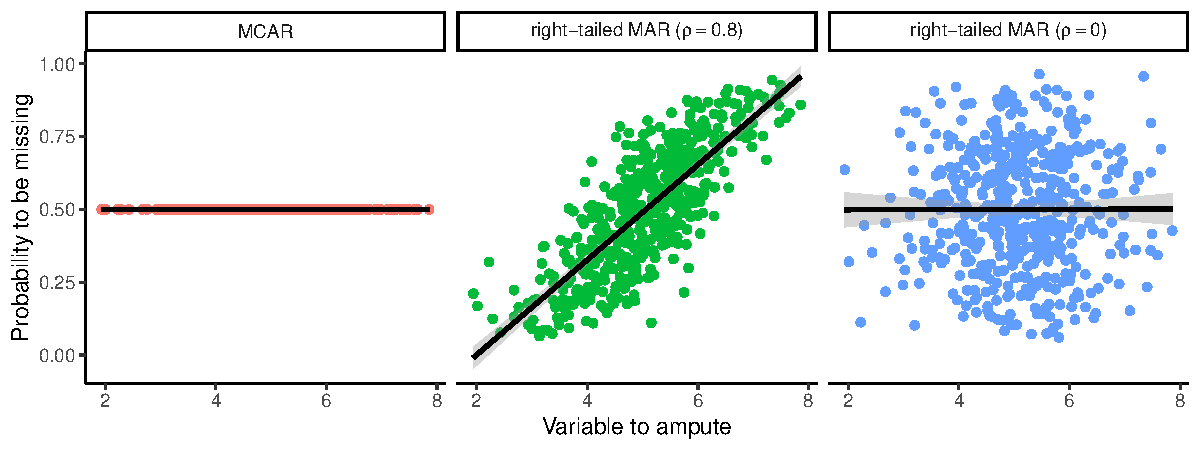
\includegraphics{plots/plot_mmech.pdf}
  }      
  \caption{Three different realizations of missingness generation for MCAR and right-tailed MAR missingness mechanisms for different levels of correlation $\rho$ between the \emph{variable to ampute} and the \emph{missingness covariate} that guide the probability to be missing. Note that the conditional probability of right-tailed MAR ($\rho=0$) mimics that of MCAR because the variable to ampute and the missingness covariate have $\rho=0$.}
    \label{Fig}
\end{figure}


% latex table generated in R 4.2.2 by xtable 1.8-4 package
% Thu Nov 17 17:52:47 2022
\begin{table}[t!]
\caption{Inferences obtained by complete case analysis (CCA) and multiple imputation over 1000 simulations. Displayed are the bias of the mean, coverage rate (cov) of the corresponding 95\% confidence interval and the confidence interval width (ciw). Imputations are generated by Bayesian linear regression imputation.}
\centering
\begin{tabular}{rlccccccc}
  \hline
 	& &\multicolumn{3}{c}{CCA} &&\multicolumn{3}{c}{imputation}	\\\cline{3-5}\cline{7-9}
 \multicolumn{2}{c}{mechanism}	& bias & cov & ciw && bias & cov & ciw \\ 
  \hline
$[\rho = .8]$ &mcar & 0.000 & 0.940 & 0.178 & & -0.000 & 0.941 & 0.160 \\ 
$[\rho = .8]$ &mar   & 0.335 & 0.000 & 0.169 & & 0.004 & 0.954 & 0.190 \\ 
$[\rho = .0]$ &mar   & 0.001 & 0.973 & 0.180 & & 0.011 & 0.939 & 0.311 \\ 
   \hline
\end{tabular}
\label{Tab}
\end{table}  




A non-ignorable or MNAR mechanism--where the unobserved values themselves may also play a role in the probability to be missing--might fall outside many studies' scope, yet could yield informative insights for daily practice. Even if an imputation method is specifically developed with ignorable missingness in mind, chances are that the method will be applied to non-ignorable empirical missingness at some point in time. After all, for every MNAR mechanism there is a MAR mechanism with equal fit and one cannot definitively verify that empirical missingness is random \citep{molenberghs2008every}. Therefore, it can be argued that MNAR is the more likely mechanism for real-life missingness scenarios. It may be wise to include MNAR missingness in the simulation study just in case: A method that performs well under MAR and some cases of MNAR may be preferable over a method that only works under MAR, and not under MNAR. Such `late-phase` methodological investigations \citep[see][]{hei22} can provide an understanding of an imputation method's robustness. Alternatively, a sensitivity analysis may provide an indication of the validity of the obtained inference, given that the assumed missingness mechanism is suspected to be invalid \citep[see e.g.][part 5]{molenberghs2014handbook}.

In addition to varying the missingness mechanisms, each simulated mechanism should be combined with different missingness patterns. Remember that missingness is only ignorable under MAR when the parameter of the data is distinct and a-priori independent from the parameter of the missing data process \citep[Corollary 6.1A]{litt20}. Under MAR missingness we assume that we may use the observed data to make inferences about the joint (observed and unobserved) data. The dependency of the procedure on the assumption under which we obtain inference is only influenced by the amount of missingness. If there is no missingness--or if there is no data, for that matter-- the inference does not depend on the assumption. Alternatively, the validity of assumptions becomes increasingly important when the missingness increases. Since we control the MAR mechanism, the assumption under which we may solve the missing data problem should hold and it is only fair to assess performance under stringent missingness conditions. We, therefore, propose to evaluate imputation methodology under several missingness proportions to emulate a realistic range in severity of the missingness problem. Depending on how the missingness mechanism interacts with the simulated data, higher missingness proportions may yield biased or invalid completed data inferences. The missingness proportions should thus be considered carefully.

The above emphasizes the need for both thorough evaluation and thorough documentation of the intended and used missingness mechanisms. Simulators must make clear which mechanisms are of interest. To be able to verify these mechanisms, simulators must also be transparent about the process that generated the missingness. For example by sharing the code or detailing the process that generated the missing values. Alternatively, missingness generation devices, such as the \texttt{mice::ampute()} function can be used to generate valid, pattern-based missingness in any structured data set \citep{mice, ampute}. Finally, simulators must include simulation conditions and evaluation parameters that make it possible to identify the proper generation of missing values. This would prevent that errors in the missingness generation would go unnoticed. 


%%%%%%%%%%%%%%%%%%%%%%%%%%

\subsection{Performance evaluation}
The evaluation criteria used to assess imputation performance vary from one simulator to another. This is not surprising as people from different fields could have a different focus on the problem at hand. There are, however, some overarching issues when assessing imputation method performance. In the first place, there are pitfalls in the evaluation of the estimates that are obtained by fitting the analysis model after imputation. For example, focusing on one performance measure over another, may yield different conclusions about imputation efficacy. In the second place, diagnostic evaluation of the generated imputations is often left out of simulation study results. Identifying problems with the imputation-generating process (e.g., an iterative imputation algorithm) may offer explanations for under-performance of imputation methods. Such evaluations, however, are typically omitted and valuable insights into the imputation method(s) may then be overlooked. 

At minimum, imputation method performance should be quantified using appropriate measures. It depends on the specifics of each simulation study which performance measures would be most suitable. If the goal is inference--not prediction--the uncertainty about estimates needs to be properly quantified. To capture this uncertainty, the standard errors of the estimates should be correctly calculated, which requires multiple imputation. The aim of multiple imputation is not to reproduce the data, but to allow for obtaining valid inference given that the data are incomplete. This means that, given the framework provided by \citet{rubi87}, and for any $(Q-\bar{Q}$, statistical properties such as bias, confidence intervals, and the coverage rate of the confidence intervals should always be studied. We therefore recommend evaluating the following points:

(i) The methods should preferably be unbiased. Note that the way bias is calculated should be carefully chosen and described, since this can greatly influence the interpretation of the results. A negligible absolute bias, for example, may already yield an almost infinite relative bias if the true value of the estimand is zero. In most cases, unbiased estimation may be expected under a MCAR missingness mechanism, which can be easily verified by including MCAR missingness in the scope of missingness investigations.

(ii) The intervals around estimates should have a valid coverage of the population (i.e. true) value. Coverage of a 95\% interval should in theory be $\geq 95$\%, where a coverage rate of 95\% would be most efficient \citep[p. 589]{neym34}. Under-coverage indicates that the procedure is not confidence valid and may lead to invalid inference. Under-coverage may occur when the estimation procedure is either biased, too liberal leading to intervals that are too narrow, or both. Over-coverage, though technically not confidence invalid, would indicate that efficiency could still be gained. In such cases, a narrower interval exists for which the method would still yield confidence valid result. 

(iii) The width of the confidence or credible interval may convey statistical efficiency, which should be considered to compare imputation methods. Wider intervals are associated with more uncertainty whereas a more narrow interval that is still properly covered indicates a sharper inference. However, inference from a wider interval that is properly covered is to be considered more valid than a more narrow interval that is not properly covered anymore. That said, with valid nominal coverage, the method that yields the narrowest interval would be most efficient. 

(iv) Resemblance to the true data values may be quantified using the root mean squared error (RMSE). We do not generally recommend the use of the RMSE as evaluation criterion, because this metric does not account for the inherent uncertainty of the missing values and it may inflate the type I error rate of statistical inferences \citep[Chapter 2.6][]{buur18}. However, if a study is aimed at obtaining predictions, and inferential validity is not of interest, the RMSE of the prediction errors (residuals) can be compared between methods. Then, the RMSE may yield valuable information about the methods' comparative efficiency in terms of accuracy and precision. 

After establishing the statistical validity of an imputation routine on the level of the estimand, it remains paramount to also study the imputation-generating process. Omitting such investigations may yield sub-optimal results. One simple example arises often in practice: generating implausible imputed values. Even though the estimation on the analysis level may be justified, some methods can yield imputations that may seem completely invalid to applied researchers. For example, one could very accurately estimate average human height by filling in negative values and values that are unrealistically large. While the obtained inference could still be valid under such imputations, the plausibility of the imputed values given the observed data should be under scrutiny. Under many circumstances, imputation methods may be realistically expected to preserve both marginal and conditional distributions with respect to the comparative truth. Imputation methods that fail to do so, should not be considered general-purpose methods. Many techniques can yield valid inferences, but techniques that sample realistic or plausible values may be preferable in practice. 

The evaluation of simulated results goes far beyond plausibility and distributional characteristics. The quality and validity of an imputation task will also rely on the relation between the missing data models, imputation models, and analysis models. When a joint model exists whose conditionals would include the imputation and analysis model, then the imputation model and analysis are said to be congenial \citep{meng94, bart2015}. The congeniality of all imputation models should be assessed, but methods to assess the suitability of imputation models and diagnose misfit often rely on visual inspection of the imputations \citep[see e.g.][]{abayomi2008diagnostics, bond16}. This makes its assessment a challenging and time-consuming endeavour in many simulation studies. 

When algorithms are used the simulator should study the validity of the algorithmic process. Many contemporary imputation techniques rely on iterative algorithms, such as the Gibbs sampler, to generate imputations. As with any iterative algorithm--but especially with imputation algorithms that are critically considered to be possibly incompatible Gibbs samplers \citep[PIGS,][]{li2012imputing}--algorithmic convergence should be carefully evaluated. \citet{ober21} demonstrate that statistical validity can happen before algorithmic convergence is reached, but this is not a guarantee. Unfortunately, there is no universal quantitative method to diagnose non-convergence in iterative imputation algorithms \citep{zhu15, ober21} and the alternative \citep[visual inspection of the imputation algorithm;][]{buur18} is neither efficient nor fail-proof. As a result, imputation algorithms may be terminated before reaching a stable state, which could yield sub-optimal imputations and under-estimated performance of the method. Problems with producing stable imputations are not exclusive to iterative imputation algorithms. Any method may run into failures of the imputation-generating process and subsequently lack results, for example due to over-parameterisation errors.

Every imputation workflow should therefore contain an evaluation of the obtained imputations. Even though inspecting each imputation may be labour-intensive due to the number of imputations generated in a simulation study, we highly recommend simulators consider the following aspects:

(i) The absence of non-convergence in the imputation-generating process is a minimum requirement for any imputation method. If non-convergence is suspected, the inference resulting from the imputations might be invalid. However, preliminary work suggests that iterative imputation algorithms could achieve inferential validity before reaching a stable state \citep{ober21}. 

(ii) The fit of the imputation model may be verified with the help of a posterior predictive check \citep[][]{nguy17, zhao22}. A straightforward posterior predictive check for imputation methodology is the multiple over-imputation of observed data values \citep{caiPPC}. If the statistical properties of the over-imputed values are equivalent to those of the observed data values, one could infer that the imputation model fits the observed part of the incomplete data reasonably well. Then, by extension, one could assume that the imputation model might be able to produce good imputations for the missing part of the data too. This over-imputation procedure is straightforward with the \texttt{overimpute()} function in \texttt{Amelia II} \citep{amelia} and the \texttt{where} argument in \texttt{mice} \citep{mice, caiPPC}.

(iii) The distributional characteristics of the imputations should be inspected for anomalies. The distribution of the incomplete data may differ greatly from the observed data. Under anything but the MCAR assumption, this can be expected. When evaluating imputations, the distributional shapes should be checked and diagnostic evaluations should be performed \citep[see][for a detailed overview of diagnostic evaluation for multivariate imputations]{abayomi2008diagnostics}. When anomalies are found, and if the imputation method is valid, there should be an explanation, especially in the controlled environment of a properly executed simulation study. 

(iv) Finally, the plausibility of the imputed values may be evaluated. Plausible imputations--imputations that could be real values if they had been observed--are not a necessary condition for obtaining valid inference. However, in practice, especially when the imputer and the analyst are different persons, plausible imputations may be a desired property. One would prefer an imputation technique to yield both valid inference and plausible imputations. It should be studied if an imputation method is prone to deliver such impractical results, and if so, under what conditions. When evaluating imputation routines, the evaluator should mention whether the routine is prone to deliver implausible values. We must note, however, that the aim of imputation should be valid inference in the first place, and plausibility in the second place. 

There are parallels between evaluating the performance and evaluating the missingness. Just like using MCAR as a condition to benchmark the validity of the missing data solution, we can use the simulation's complete data (i.e. without missing values) as an upper limit for our performance evaluation. In addition, the simulator should also perform complete case analysis, i.e. analysis on the incomplete data without solving for the missingness. We know the theoretical properties of complete case analysis, which makes the ad hoc technique useful as a lower limit for evaluating imputation performance. Complete case analysis may, therefore, serve as a benchmark method against which imputation performance should be evaluated. Realistically, the simulator would expect the imputation solution to perform not worse than the complete case analysis and, preferably, mimic the complete data results. Moreover, pairing complete case analysis with MCAR and MAR mechanisms allows the simulator to evaluate the impact of the missing data generation process under the chosen analysis model and to identify the unintentional generation of accidental MNAR. 

Last, when the simulator is on the verge of drawing conclusions about the performance of the imputation methodology, the performance should be carefully qualified. Comparing the performance of an imputation routine given a population (or true) parameter allows for quantitative evaluation. Yet, in order to pose qualitative statements about the performance on simulated conditions, comparative methodology is required. For example, when claiming that imputation performance is unacceptable when deviations from normality become rather stringent, such performance is highly dependent on the simulation conditions that are used. For a well-balanced judgment about the severity of the performance drop, comparative simulations with e.g. non-parametric models should be executed. A method may perform badly, but if it still outperforms every other approach, it may yet be of great practical relevance.


%%%%%%%%%%%%%%%%%%%%%%%%%%
%% DISCUSSION
%%%%%%%%%%%%%%%%%%%%%%%%%%

\section{Suggested course of action}

We encourage simulators to carefully consider and document their choices in the evaluation of imputation methodology. Simulation studies should not only be well-executed, but also properly reported. For example, the inconsistent display of simulation conditions may impact the objectivity of meta-evaluations over imputation methods, as one method's performance may appear to be favourable because of less stringent simulation conditions. This may ultimately lead to statisticians recommending a less efficient method to applied researchers, thereby limiting the efficiency of the imputation approach and unnecessarily lowering the statistical power. Simulators should therefore be explicit in the descriptions of their evaluations. However, deciding what and how to report may be challenging. The simulation design could be presented textually, in a flow chart or as a block of pseudo-code, whereas missingness mechanisms could be written as a function of the data or displayed graphically. Ideally, the evaluations should be supplemented by an online repository with all of the data and code required to reproduce the simulation results. To aid simulators in reporting and move towards standardization in evaluation, we provide a draft version for reporting guidelines in Appendix A.1 (also available from \underline{www.gerkovink.com/evaluation}). We invite the readers of this paper to contribute to its development. 

We aim to elicit critical thinking about incomplete data simulation and to establish a common ground for the evaluation of imputation routines. Such a common ground would be the basis of a standardized evaluation. This would allow for fairer and more efficient comparisons between imputation techniques. Ultimately, it would be desirable to evaluate every imputation routine against the same standardized set in order to quantify the statistical properties across imputation routines. If properly executed, such evaluations would allow for careful matching of imputation methodologies to new missing data problems. 


%%%%%%%%%%%%%%%%%%%%%%%%%%
%% APPENDICES
%%%%%%%%%%%%%%%%%%%%%%%%%%

\begin{acknowledgement}
We thank the Amices team for the fruitful discussions.
\end{acknowledgement}
\vspace*{1pc}

\noindent {\bf{Conflict of Interest}}

\noindent {\it{The authors have declared no conflict of interest.}}

\newpage

\section*{Appendix}

\subsection*{A.1.\enspace Reporting guidelines}

Table \ref{table:check} provides a checklist for reporting on imputation methodology evaluations. We have structured the checklist according to simulation study reporting format proposed by \citet{morr18}.  

\begin{table}[ht!]
\caption{Checklist for reporting on imputation methodology evaluations.}
\label{table:check}
\begin{tabular}{ll}
\hline
$\square$ & \textbf{Aims}                                                                                  \\
  & e.g. simulation scope                                                                          \\ \cline{2-2} 
  & $\square$ simulation design (incl. pseudo-code or flow diagram)                                        \\
  & $\square$ required level of precision (incl. number of simulation   repetitions)                       \\ \hline
$\square$ & \textbf{Data-generating mechanisms}                                                            \\
  & e.g. data generation and missingness generation                                                \\ \cline{2-2} 
  & $\square$ data source (incl. model-based or design-based, sampling   variance)                         \\
  & $\square$ data characteristics (incl. multivariate relations and data   structures such as clustering) \\
  & $\square$ missingness mechanisms (incl. type or functional form of the   missing data model)           \\
  & $\square$ missingness patterns (incl. missingness proportion)                                          \\ \hline
$\square$ & \textbf{Estimands}                                                                             \\
  & e.g. complete data target                                                                      \\ \hline
$\square$ & \textbf{Methods}                                                                               \\
  & e.g. missing data methods, analytic method and inference pooling rules                                    \\ \cline{2-2} 
  & $\square$ imputation methods (incl. parameters such as the number of   imputations)                    \\
  & $\square$ estimation method (incl. reference methods such as complete   case analysis)                 \\
  & $\square$ methods used to construct standard errors and confidence intervals \\ 
  & $\;\;$ $-$ Such as rules by \citet{rubi87}, \citet{bar99}, \citet{rei03}, etc.    \\ \hline
$\square$ & \textbf{Performance measures}                                                           \\      
  & e.g. evaluation of estimates and imputed values                                                \\ \cline{2-2} 
  & $\square$ statistical properties (incl. comparative performance, if   applicable)                      \\
  & $\square$ validity of imputations (incl. imputation model fit and distributional characteristics)    \\ 
  & $\;\;$ $-$ Does the imputation model fit well to the observed values? (e.g. posterior predictive check)   \\ 
  & $\;\;$ $-$ Are there unrealistic values in the data? (e.g. negative where positive expected)   \\ 
  & $\;\;$ $-$ Are there implausible combinations in the data? (e.g. pregnant grandfathers)   \\ \hline
  
\end{tabular}
\end{table}



%%%%%%%%%%%%%%%%%%%%%%%%%%
%% REFERENCES
%%%%%%%%%%%%%%%%%%%%%%%%%%
\bibliography{bibliography}
\bibliographystyle{apalike}

% \begin{thebibliography}{10}
% \bibitem[Bauer and Bauer(1994)Bauer, P. and Bauer, M.M.]{bib1}Bauer, P. and Bauer, M. M. (1994). Testing equivalence simultaneously for location and dispersion of two normally distributed populations. \textit{Biometrical Journal} \textbf{36}, 643--660.
% \bibitem[Farrington, C. P. and Andrews, N. (2003)]{bib2}Farrington, C.P. and Andrews, N. (2003). Outbreak detection:
% Application to infectious disease surveillance. In: Monitoring the Health of Populations (eds. R. Brookmeyer and D. F. Stroup), Oxford University Press, Oxford,\break 203--231.
% \bibitem[Rencher(1998)Rencher, A.C.]{bib3}Rencher, A. C. (1998). \textit{Multivariate Statistical Inference and Applications}. Wiley, New York. 
% \end{thebibliography}
% \newpage
% \phantom{aaaa}
\end{document}
